\documentclass{beamer}

\usepackage{graphicx}
\usepackage{hyperref}
\usepackage[utf8]{inputenc}
\usepackage[german,english]{babel}
\usepackage[T1]{fontenc}
%\usepackage[english]{babel}
\usepackage{listings}
\usepackage{xcolor,url}
\usepackage{amssymb}
\usepackage{amsmath}
\usepackage{amsfonts}
\usepackage{ifthen}
\usepackage{tcolorbox}
\usepackage{tikz}
\usepackage{upgreek}
\usepackage{dsfont}
\usepackage{framed, color}

\usepackage{metricsbeamer} % using the metric beamer style

\DeclareMathAlphabet{\mathcalbf}{OMS}{cmsy}{b}{n}
%\newcommand{\dd}{\text{d}}
\newcommand{\del}{\partial}

% The command to define a subsection is '\subsec{}' and NOT '\subsection'.
% This code generates the bar. Don't edit.
\newcommand{\midbarnew}{}
\newcommand{\subsec}[1]
{
  \ifthenelse{\equal{#1}{}}
  {\renewcommand{\midbarnew}{} \subsection{}}
  {\renewcommand{\midbarnew}{ $\mid$ } \subsection{#1}}
}

% change the pictures here, if necessary. logobig and logosmall are the internal names
% for the pictures: do not modify them, just change "hulogo" and "logo". Pictures must be 
% supplied as JPEG, PNG or PDF
%########################################

\pgfdeclareimage[height=2cm]{logobig}{hulogo} % use hucase instead for the Humboldt-Case Logo
\pgfdeclareimage[height=1cm]{logosmall}{hulogo}

% use this number to modify the scaling of the headline on titlepage
\def\titlescale{1.3}


\def\authora{Philipp Töpfer}	% First Author
%\def\affa{Humboldt-Universität zu Berlin, Institut für Physik} % First Author's Affiliation
%\def\authorb{Her Name}  % Second Author
%\def\affb{Humboldt-Universität zu Berlin} % Second Author's Affiliation
%\def\authorc{His Name}  % Third Author
%\def\affc{Humboldt-Universität zu Berlin} % Third Author's Affiliation

\def\linka{}	% Link to your institution's/ personal website
\def\linkb{}
\def\linkc{}
\def\email{\href{mailto:your.email@address.com}{your.email@address.com}}	% Your email address

\title[Strings on the lattice and AdS/CFT]{\centering Lattice discretisation of the Green-Schwarz superstring and AdS/CFT \\}
\institute{Humboldt-Universität zu Berlin \\ Emmy Noether Research Group}

% - - - - - - - - - - - - - - - - - - - - - - - - - - - - - - - - - -


%Start of the document
\begin{document}
\Section{}

\frame[plain]{% create the titleslide, layout controlled in metricsbeamer
\vspace{-1.5cm}	\titlepage
}

\Section{Introduction}

\frame{% how to print
\frametitle{Outline}

\begin{tcolorbox}[colback=white!95!black, colframe=white!90!black]
\begin{center}
Study the \textcolor{blue!90}{AdS/CFT duality} \textcolor{blue!95!black}{numerically} at hand of the \textcolor{blue!90}{cusp anomaly function} from a \textcolor{blue!90}{string theory perspective}
\end{center}
\end{tcolorbox}
\hfill \vspace{1mm}



\begin{itemize}
\item<2-> Motivation
\item<2-> Cusp anomaly function
\item<2-> AdS/CFT duality
\item<2-> String theory framework
\item<2-> Numerical approach
\end{itemize}

}

%###############################################

\Section{Motivation}

\frame{
\frametitle{Motivation}

\begin{itemize}
\item<1-> Good predictions on the real world via QCD
\item<1-> Fundamental aim: particle masses as functions of parameters\\
\begin{center} $m_{\rm p} = f(\alpha_{\rm s},\alpha,\mu_{\rm reg},\ldots)$ \end{center}
\item<2-> Gain more insights on QCD $\leftrightarrow$ study more symmetric model %($\mathcal{N}=4$ SYM)
\item<2-> $\mathcal{N}=4$ SYM: 
\begin{itemize}
\item no massive particles
\item measure scaling dimensions of local operators and Wilson loops
\end{itemize}
\item<3-> Twist two operators:\\
scaling dimension $\Delta_{S} = 2+S+ \gamma_{S}$
\end{itemize}
}

%################################################

\Section{Cusp anomaly function}

\begin{frame}
% mp left
\begin{minipage}[t]{0.5\linewidth}
\begin{tcolorbox}[colback=white!95!black, colframe=white!90!black]
\begin{center}
\vspace{2.5mm}
Wilson loop with cusp
\vspace{2mm}
\end{center}
\end{tcolorbox}
%
\begin{tcolorbox}[colback=white!95!black, colframe=white!90!black]
\begin{center}
$\langle \mathcal{W}[\mathcal{C_{\rm cusp}}]\rangle \sim e^{-\frac{\color{blue}{f(g)}}{2}\vert \phi\vert \ln \frac{L}{\epsilon}}$
\end{center}
\end{tcolorbox}
\end{minipage}
%
% mp center
%
\begin{minipage}[t]{0.05\linewidth}
\begin{center}
\vspace{1.5mm}
$\Leftrightarrow$
\end{center}
\end{minipage}
%
% mp right
%
\begin{minipage}[t]{0.4\linewidth}
\begin{tcolorbox}[colback=white!95!black, colframe=white!90!black]
\begin{center}
anomalous dimension $\gamma_{S}$
\end{center}
\end{tcolorbox}
%
\begin{tcolorbox}[colback=white!95!black, colframe=white!90!black]
\begin{center}
\vspace{1mm}
$\gamma_{S} \simeq {\color{blue}f(g)} \ln S$
\vspace{1mm}
\end{center}
\end{tcolorbox}
\end{minipage}
%
%
%
\only<1>{
\begin{center}
\begin{tikzpicture}[thick,scale=0.5, every node/.style={scale=0.7}]
\node[anchor=south west,inner sep=0] (image) at (0,0) {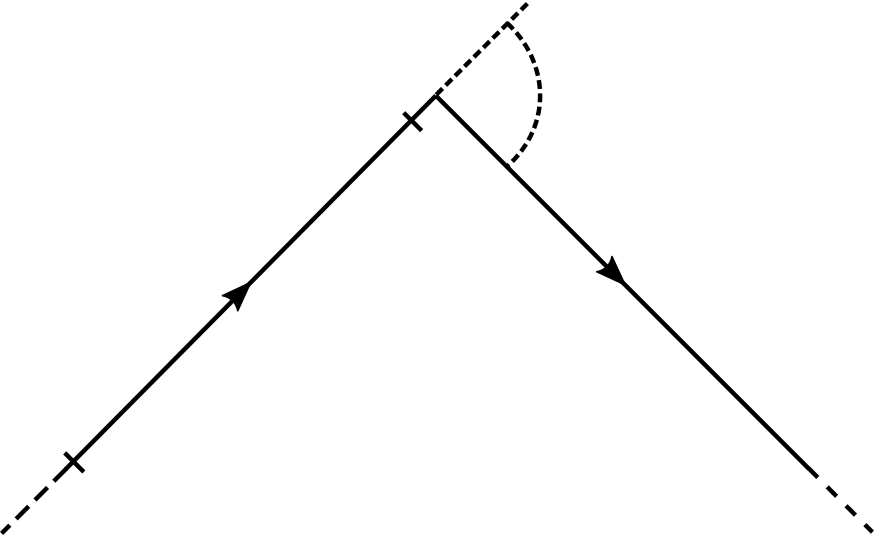
\includegraphics[width=0.8\textwidth]{W_cusp.png}};
\begin{scope}[x={(image.south east)},y={(image.north west)}]
\node [anchor=west] at (0.69,0.3) {$\mathcal{C_{\rm cusp}}$};
\node [anchor=south] at (0.072,0.14) {$L$};
\node [anchor=south] at (0.45,0.78) {$\epsilon$};
\node [anchor=west] at (0.62,0.82) {$\phi$};
%\draw[help lines,xstep=.1,ystep=.1] (0,0) grid (1,1);
%\foreach \x in {0,1,...,9} { \node [anchor=north] at (\x/10,0) {0.\x}; }
%\foreach \y in {0,1,...,9} { \node [anchor=east] at (0,\y/10) {0.\y}; }
\end{scope}
\end{tikzpicture}
\end{center}
}
%
%
\only<2>{
\begin{center}
via cusp anomaly function
\end{center}
\begin{minipage}{0.65\linewidth}
\begin{tikzpicture}[thick,scale=0.5, every node/.style={scale=0.7}]
\node[anchor=south west,inner sep=0] (image) at (0,0) {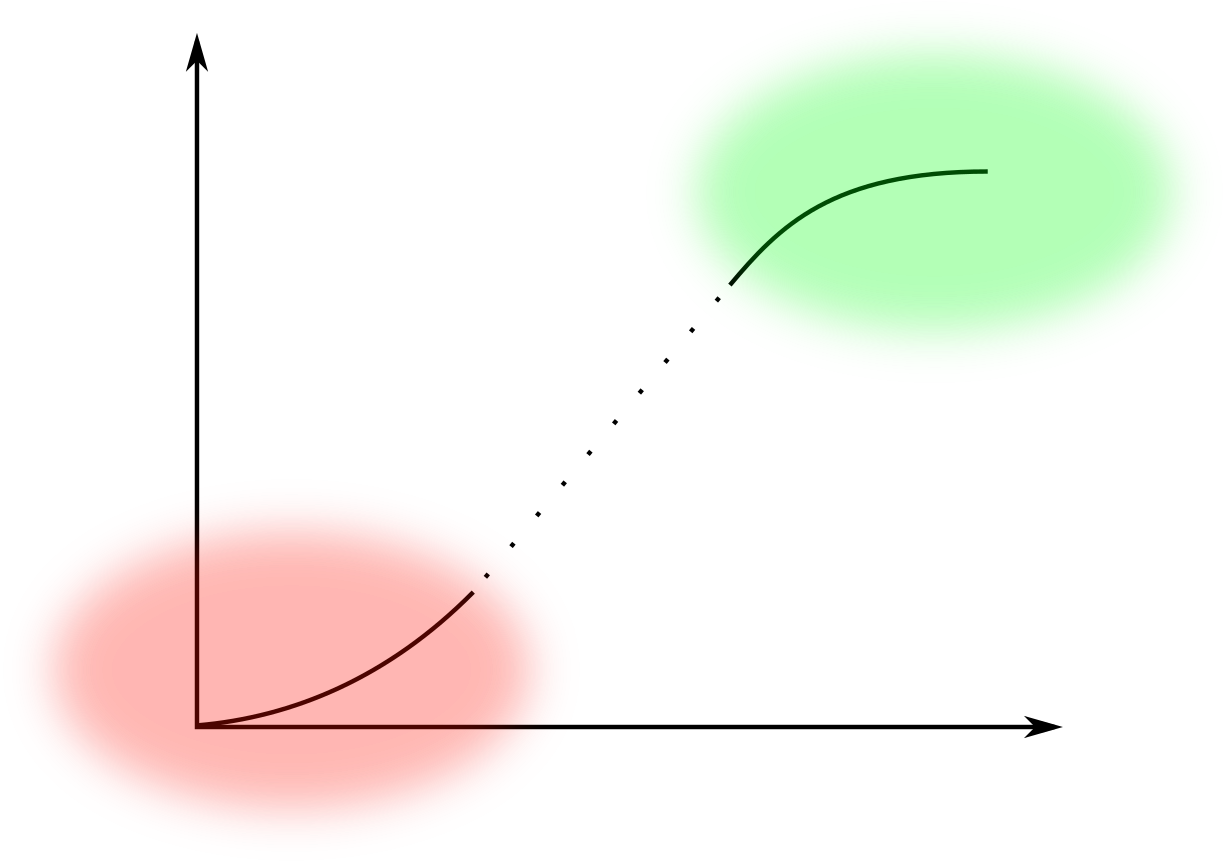
\includegraphics[width=1.1\textwidth]{cusp_anom.png}};
\begin{scope}[x={(image.south east)},y={(image.north west)}]
\node [anchor=east] at (0.15,0.92) {$\color{blue} f(g)$};
\node [anchor=north] at (0.85,0.15) {$\color{blue} g$};
\node [anchor=south] at (0.75,0.8) {\footnotesize pert. string $\sigma$-model};
\node [anchor=north] at (0.22,0.17) {\footnotesize pert. gauge theory};
\node [anchor=east] at (0.5,0.6) {\textcolor{red}{\footnotesize Integrability}};
\node [anchor=west] at (0.5,0.5) {\textcolor{red}{\footnotesize non-pert. methods}};
%\draw[help lines,xstep=.1,ystep=.1] (0,0) grid (1,1);
%\foreach \x in {0,1,...,9} { \node [anchor=north] at (\x/10,0) {0.\x}; }
%\foreach \y in {0,1,...,9} { \node [anchor=east] at (0,\y/10) {0.\y}; }
\end{scope}
\end{tikzpicture}
\end{minipage}
%
%
\begin{minipage}{0.3\linewidth}
Here ${\color{blue}g} \equiv \frac{\sqrt{\lambda}}{4\pi} $ \\[2mm]
$\lambda = g_{\rm YM}^{2}N = \frac{R^{4}}{\alpha'^{2}}$

\end{minipage}
}
\end{frame}

%################################################

\Section{AdS/CFT duality}
\frame{
\frametitle{AdS/CFT duality}

\begin{tcolorbox}[colback=white!95!black, colframe=white!90!black]
\begin{center}
conformal field theory (CFT)
\end{center}
\end{tcolorbox}
%
\begin{equation*}
\uparrow \qquad \textit{dynamically equivalent to} \qquad \downarrow
\end{equation*}\hspace{1mm}
%
%
\begin{tcolorbox}[colback=white!95!black, colframe=white!90!black]
\begin{center}
string theory on background containing Anti-de Sitter (AdS) space as a factor
\end{center}
\end{tcolorbox}

}

%############################################

\frame{
\textbf{Most symmetric setting similar to QCD:} \\[0.3cm]

\begin{tcolorbox}[colback=white!95!black, colframe=white!90!black]
\begin{minipage}{0.70\linewidth}
\begin{center}
\textbf{$\mathcalbf{N}=\mathbf{4}$ SYM}\\
 in 4d, $( g_{\rm YM}, N)$
\end{center}
\end{minipage}
\begin{minipage}{0.20\linewidth}
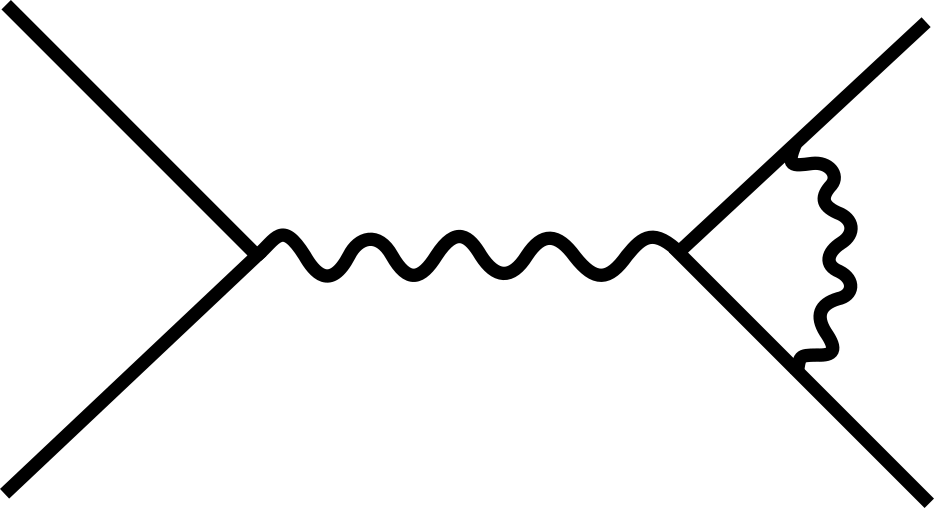
\includegraphics[scale=0.15]{feynm.png}
\end{minipage}


\end{tcolorbox}
%
\begin{equation*}
\uparrow \qquad \textit{dynamically equivalent to} \qquad \downarrow
\end{equation*}\hspace{1mm}
%
%
\begin{tcolorbox}[colback=white!95!black, colframe=white!90!black]
\begin{minipage}{0.65\linewidth}
\begin{center}
\textbf{Type IIB superstring theory}\\
on $AdS_{5}\times S^{5}$,  $(g_{\rm s},R)$
\end{center}
\end{minipage}
\begin{minipage}{0.15\linewidth}
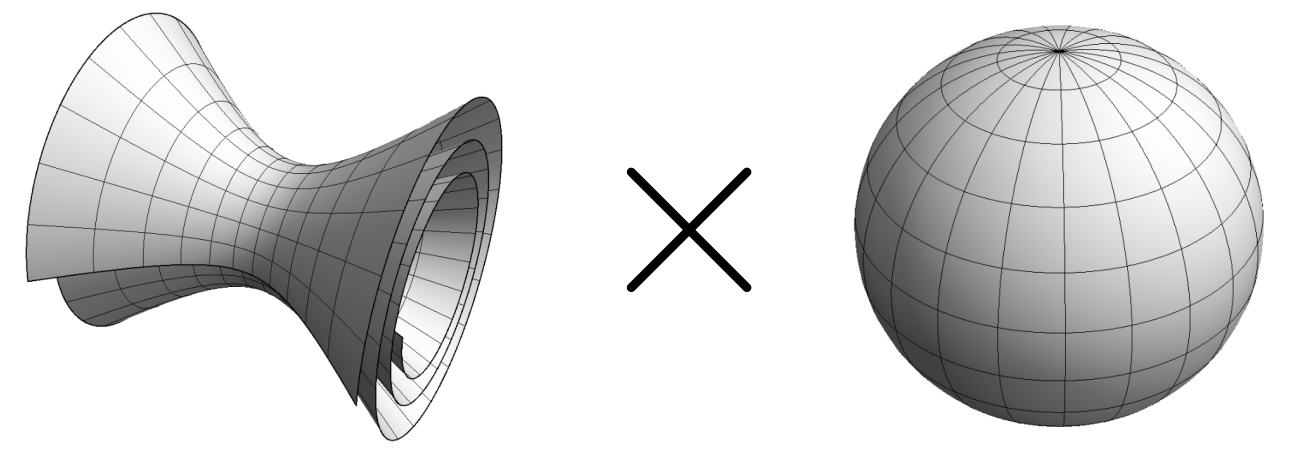
\includegraphics[scale=0.15]{AdS_S.png}
\end{minipage}
\end{tcolorbox}

}

%##############################################

\frame{
\begin{minipage}{0.25\linewidth}
\begin{tcolorbox}[colback=white!95!black, colframe=white!90!black]
\begin{center}\vspace{3mm}
\textbf{$\mathcalbf{N}=\mathbf{4}$ SYM}
\vspace{3mm}
\end{center}
\end{tcolorbox}
%
%
\begin{tcolorbox}[colback=white!90!red, colframe=white!90!black]
\begin{center}
\vspace{5mm}
$\Uparrow$\\
\textbf{AdS/CFT}\\
$\Downarrow$\\
\vspace{5mm}
\end{center}
\end{tcolorbox}
%
%
\begin{tcolorbox}[colback=white!95!black, colframe=white!90!black]
\begin{center}
\textbf{Type IIB strings}
\end{center}
\end{tcolorbox}
\end{minipage}
%
%
%
\begin{minipage}{0.73\linewidth}
\begin{tcolorbox}[colback=white!95!blue, colframe=white!90!black]
\begin{center}
Wilson loop
\end{center}
$\langle \mathcal{W}[\mathcal{C}]\rangle = \frac{1}{N}{\rm Tr}\,\mathcal{P}\,e^{\oint \left(iA_{\mu}\dot{x}^{\mu}+\phi_{i}\dot{y}^{i}\right) {\rm d}s }$
\end{tcolorbox}
\begin{center}
\begin{tikzpicture}[thick,scale=0.5, every node/.style={scale=0.7}]
\node[anchor=south west,inner sep=0] (image) at (0,0) {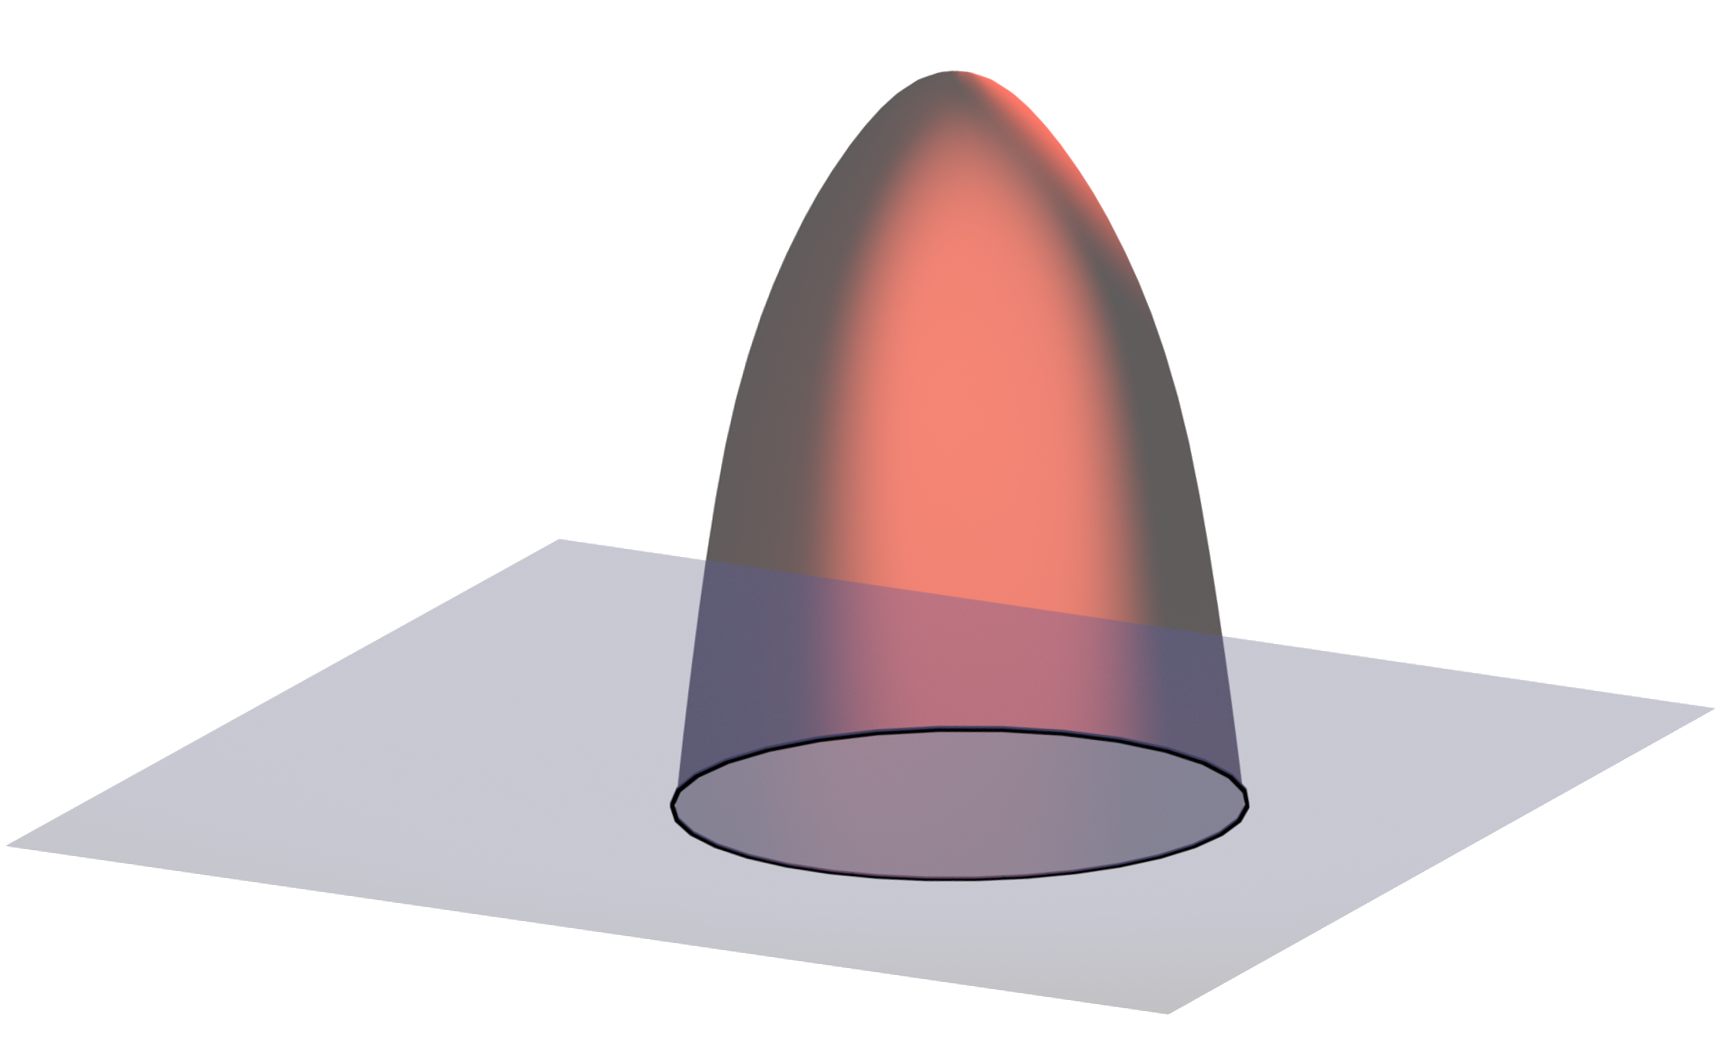
\includegraphics[width=0.7\textwidth]{Wilson_loop_worldsheet1.png}};
\begin{scope}[x={(image.south east)},y={(image.north west)}]
\node [anchor=west] at (0.6,0.1) {$\mathcal{C}$};
%\node [anchor=west] at (0.8,0.6) {$\widetilde{\Sigma}$};
%\node [anchor=west] at (0.95,0.1) {$z$};
%\draw[help lines,xstep=.1,ystep=.1] (0,0) grid (1,1);
%\foreach \x in {0,1,...,9} { \node [anchor=north] at (\x/10,0) {0.\x}; }
%\foreach \y in {0,1,...,9} { \node [anchor=east] at (0,\y/10) {0.\y}; }
\end{scope}
\end{tikzpicture}
\end{center}
%
%
%
\begin{tcolorbox}[colback=white!95!blue, colframe=white!90!black]
\vspace{1mm}
$\!\!Z_{\rm string}[\mathcal{C}]\!=\! \int \mathcal{D}X\mathcal{D}h\, e^{-S_{\rm string}(X,h)} \!\sim\! e^{-A(\mathcal{C})} $ \\
\vspace{-1mm}
\end{tcolorbox}
\end{minipage}

}

%###############################################

\frame{
\frametitle{Cusp anomaly of $\mathcalbf{N}=\mathbf{4}$ SYM from string theory}
\begin{minipage}{0.6\linewidth}
vev of light-like cusped Wilson loop\\
\begin{tcolorbox}[colback=white!95!black, colframe=white!90!black]
$\langle\mathcal{W}[\mathcal{C}_{\rm cusp}]\rangle \sim e^{\frac{f(g)}{2}\vert\phi\vert \ln \frac{L}{\epsilon}}$
\end{tcolorbox}
\end{minipage}
%
\begin{minipage}{0.35\linewidth}
\begin{center}
\begin{tikzpicture}[thick,scale=0.9, every node/.style={scale=0.7}]
\node[anchor=south west,inner sep=0] (image) at (0,0) {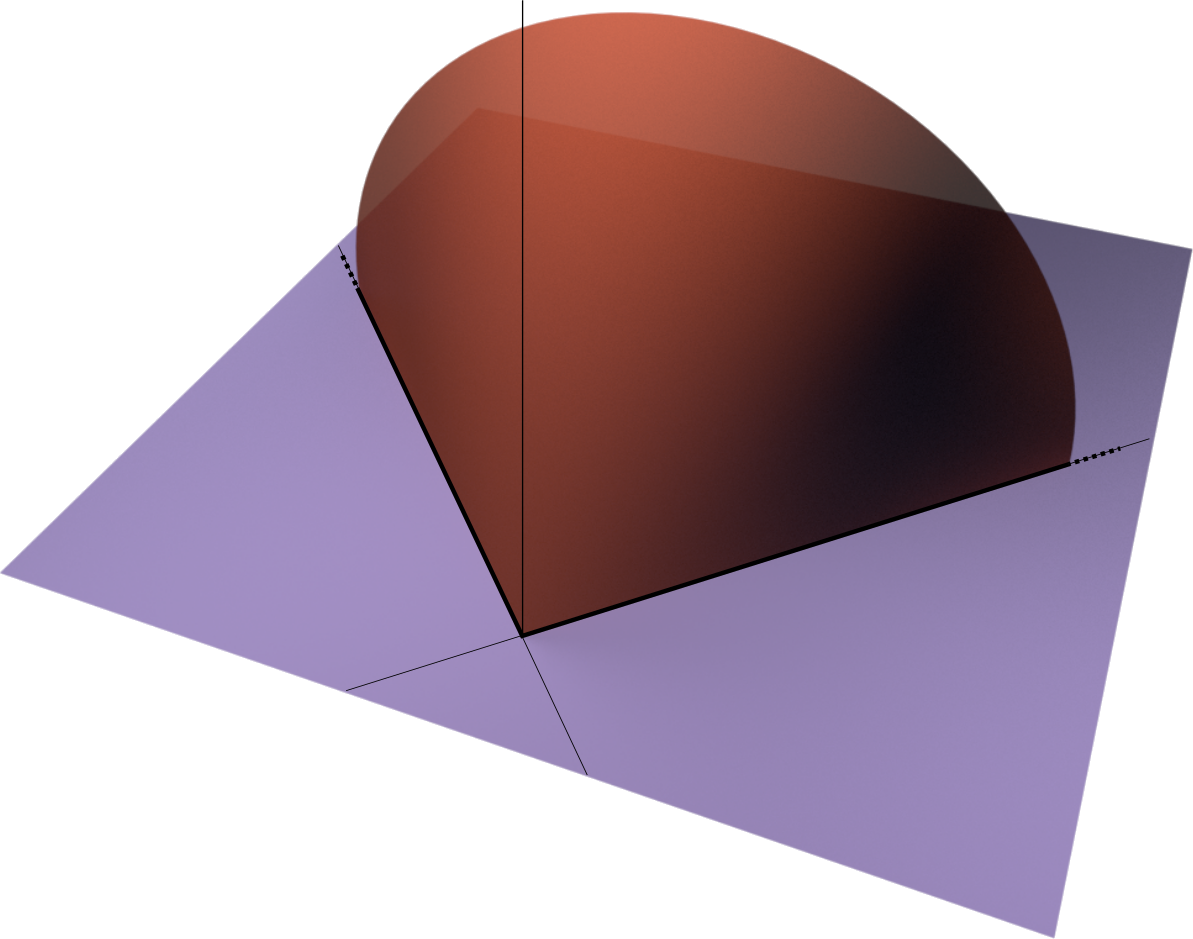
\includegraphics[width=1.2\textwidth]{cusp_worldsheet_vec.png}};
\begin{scope}[x={(image.south east)},y={(image.north west)}]
\node [anchor=north] at (0.6,0.37) {$\mathcal{C}_{\rm cusp}$};
%\draw[help lines,xstep=.1,ystep=.1] (0,0) grid (1,1);
%\foreach \x in {0,1,...,9} { \node [anchor=north] at (\x/10,0) {0.\x}; }
%\foreach \y in {0,1,...,9} { \node [anchor=east] at (0,\y/10) {0.\y}; }
\end{scope}
\end{tikzpicture}
\end{center}
\end{minipage}
%
\begin{center}
$\Updownarrow$  \textcolor{red}{AdS/CFT}
\end{center}
%
\begin{tcolorbox}[colback=white!95!black, colframe=white!90!black]
$Z_{\rm cusp} = \int \mathcal{D}\delta X \, \mathcal{D}\delta \mathit{\Psi}\; e^{-S_{\rm IIB}(X_{\rm cl}+\delta X, \delta \mathit{\Psi})} = e^{-\frac{f(g)}{2}\frac{V_{2}}{4}}$
\end{tcolorbox}
String partition function with cusp vacuum $\left( V_{2}=\int {\rm d}t{\rm d}s \right)$

}

%##############################################################

\Section{String theory framework}

\frame{
\frametitle{Green-Schwarz string in AdS light-cone gauge}

\begin{itemize}
\item Sigma-model in $AdS_{5}\times S^{5}$ with RR flux\vspace{2mm}
$S = g \int \dd\tau \dd \sigma\,\left[ G_{\mu\nu} \del X^{\mu} \del X^{\nu} + \bar{\!\mathit{\Theta}} \Gamma (D+F_{5}) \mathit{\Theta}\del X + \ldots \right]$\vspace{1mm}
\begin{flushright}
\footnotesize [Metsaev Tseytlin 1998]
\end{flushright}

\item Fix $\kappa$-symmetry and apply bosonic light-cone gauge \\
$\Rightarrow$ action at most quartic in complex Grassmann fields $\theta^{i}, \eta^{i}$

\end{itemize}
}

%###############################################################

\begin{frame}
\frametitle{Green-Schwarz string in null-cusp background}

\begin{itemize}
\item In Poincaré patch\vspace{2mm}
$\dd s^{2}_{AdS_{5}} = \frac{\dd z^{2} + \dd x^{+}\dd x^{-} + \dd x^{*}\dd x}{z^{2}}, \quad x^{\pm}=x^{3}\pm x^{0}, \quad x=x^{1}+ix^{2}$\vspace{2mm}
classical solution $\big(\tau,\sigma \in (0,\infty)\big)$: surface\vspace{2mm}
\begin{center}
$z = \sqrt{\frac{\tau}{\sigma}},\quad x^{+}=\tau,\quad x^{-}= -\frac{1}{2\sigma}$ 
\end{center}
\vspace{2mm}
bounded by a null cusp \\ ($AdS_{5}$ boundary at $0=z^{2}=-2x^{+}x^{-}$)
%
\item expand around classical solution + \\{\small $(\tau,\sigma) \to (t,s)=(\ln \tau,\ln \sigma)$}\\
\vspace{2mm}
{\small $S_{\rm cusp} = g\int \dd t\dd s\, \mathcal{L}_{\rm cusp}$}


\end{itemize}
\only<1>{
\vspace{-26mm}
%\begin{flushright}
\hspace{7.4cm}\begin{tikzpicture}[thick,scale=0.9, every node/.style={scale=0.7}]
\node[anchor=south west,inner sep=0] (image) at (0,0) {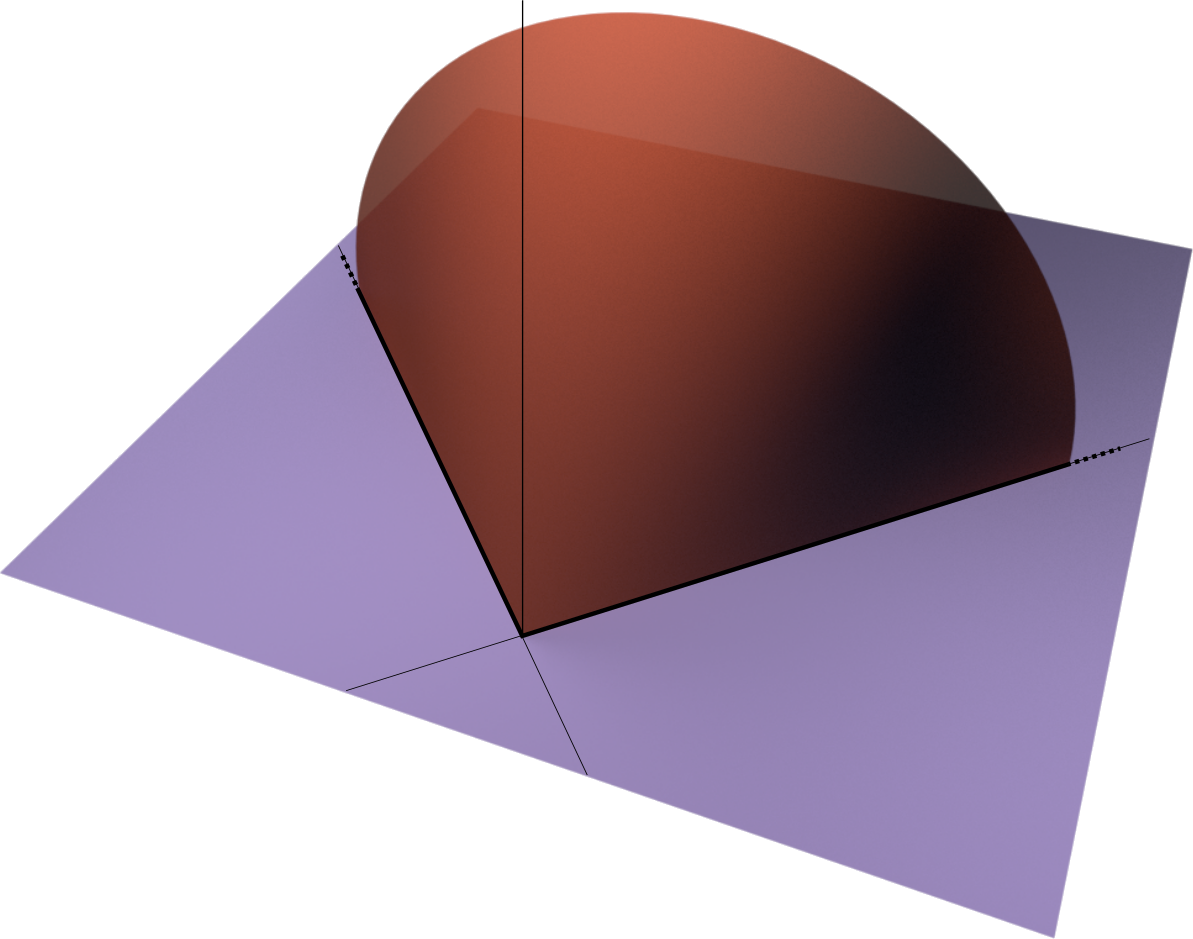
\includegraphics[width=0.5\textwidth]{cusp_worldsheet_vec.png}};
\begin{scope}[x={(image.south east)},y={(image.north west)}]
\node [anchor=north] at (0.6,0.37) {$\mathcal{C}_{\rm cusp}$};
\node [anchor=east] at (0.43,1.0) {$z$};
\node [anchor=east] at (0.28,0.75) {$x^{+}$};
\node [anchor=west] at (0.95,0.53) {$x^{-}$};
%\draw[help lines,xstep=.1,ystep=.1] (0,0) grid (1,1);
%\foreach \x in {0,1,...,9} { \node [anchor=north] at (\x/10,0) {0.\x}; }
%\foreach \y in {0,1,...,9} { \node [anchor=east] at (0,\y/10) {0.\y}; }
\end{scope}
\end{tikzpicture}
%\end{flushright}
	}
\end{frame} 

%########################################################

\frame{
\frametitle{Green-Schwarz string in null-cusp background}
linearising quartic fermion contributions
{\small \begin{align*}
\mathcal{L}_{\rm cusp} &=  {\left\vert \partial_t {x} + {\tfrac{m}{2}}{x} \right\vert}^2 + \tfrac{1}{{ z}^4}{\left\vert \partial_s {x} -\tfrac{m}{2}{x} \right\vert}^2 + \left(\partial_t {z}^M + \tfrac{m}{2}{z}^M \right)^2 \\ &\quad+ \frac{1}{{ z}^4} \left(\partial_s {z}^M -\tfrac{m}{2}{z}^M\right)^2
+ \phi^2 +\left( \phi_{I}\right)^{2} + \mathit{\Psi}^T \mathcal{O}_{\rm F} \mathit{\Psi} 
\end{align*}}

\only<1>{
\begin{itemize}
\item 8 bosonic coordinates: {\small $x,x^{*},z^{M}\;(M=1,\ldots,6),\; z=\sqrt{z_{M}z^{M}}$}
\item 17 auxiliary fields {\small $\phi, \phi_{I}$ \small $(I=1,\ldots,16)$}
\item 8 fermionic variables {\small $\mathit{\Psi} \equiv (\theta^{i},\theta_{i},\eta^{i},\eta_{i})$, $\theta^{i}=\theta_{i}^{\dagger}$, $\eta^{i}= \eta_{i}^{\dagger}$, $(i=1,\ldots,4)$}
\end{itemize}
	}
	
\only<2>{
{\footnotesize
\vspace{-8mm}
\begin{flalign*}
\!\!\!\!\!\!\!\!\!\!\!\!\!\!\!\!
\mathcal{O}_{\rm F} & =\begin{pmatrix}
0 & i \mathds{1}_{4}\partial_{t} &\!\!\!\!\! -i\rho^{M}\left(\partial_{s}+\frac{m}{2}\right)\frac{{z}^{M}}{{z}^{3}} & 0\\
i \mathds{1}_{4}\partial_{t} & 0 & 0 & \!\!\!\!\!-i\rho_{M}^{\dagger}\left(\partial_{s}+\frac{m}{2}\right)\frac{{z}^{M}}{{z}^{3}}\\
i\frac{{z}^{M}}{{z}^{3}}\rho^{M}\left(\partial_{s}-\frac{m}{2}\right) & 0 & \!\!\!\!\!2\frac{{z}^{M}}{{z}^{4}}\rho^{M}\left(\partial_{s}{x}-m\frac{{x}}{2}\right) & i \mathds{1}_{4}\partial_{t}-A^{T}\\
0 & \!\!\!\!\! i\frac{{z}^{M}}{{z}^{3}}\rho_{M}^{\dagger}\left(\partial_{s}-\frac{m}{2}\right) &i \mathds{1}_{4}\partial_{t}+A & \!\!\!\!\!\!\!\! -2\frac{{z}^{M}}{{z}^{4}}\rho_{M}^{\dagger}\left(\partial_{s}{x}^\ast-m\frac{{x}}{2}^\ast\right)
\end{pmatrix}~,
\raisetag{-8pt}
\end{flalign*}\\\vspace{2mm}
%
\small
$A=-\frac{\sqrt{6}}{z}\phi \mathds{1}_{4} + \frac{1}{z}\tilde{\phi}+\frac{1}{z^{3}}\rho^\ast_{N}\tilde{\phi}^{T}\rho^{L}z^{N}z^{L}+\mathrm{i}\frac{z^{N}}{z^2}\rho^{MN}\partial_{t}z^{M}$
}
	}	
	
}

%#################################################
\Section{Numerical approach}

\begin{frame}
\frametitle{Numerical approach}

requires calculating expectation values\vspace{2mm}
{
%\begin{align*}
\begin{tcolorbox}[colback=white!95!black, colframe=white!90!black]
\begin{center}
$Z_{\rm cusp} = \int \mathcal{D}\delta X\mathcal{D}\delta \mathit{\Psi} \; e^{-S_{\rm cusp}} = e^{-\frac{f(g)}{2}\frac{V_{2}}{4}}$
\end{center}
\end{tcolorbox} %\\
\begin{center}
$\Downarrow \qquad \qquad \Downarrow$
\end{center}
\begin{tcolorbox}[colback=white!95!black, colframe=white!90!black]
\begin{align*}
\fcolorbox{white!70!black}{white!80!blue}{$\langle S_{\rm cusp} \rangle $} &= \frac{1}{Z_{\rm cusp}} \int \mathcal{D}\delta X\mathcal{D}\delta \mathit{\Psi} \; S_{\rm cusp} e^{-S_{\rm cusp}} \\
&= -g \frac{\dd \ln Z_{\rm cusp}}{\dd g} = \fcolorbox{white!70!black}{white!80!blue}{$g f'(g) \frac{V_{2}}{8}$}
\end{align*}
\end{tcolorbox}
}
\end{frame}

%########################################################

\begin{frame}
\frametitle{Lattice discretisation}
\begin{minipage}{0.65\linewidth}
\begin{tcolorbox}[colback=white!95!black, colframe=white!90!black]
{\small ${\!\!\!\!\!\!\!\langle A \rangle = \tfrac{1}{Z}\int \mathcal{D}\phi\, A[\phi]e^{-S[\phi]}, \quad Z=\int \mathcal{D}\phi\,e^{-S[\phi]}}$}
\end{tcolorbox}% \vspace{2mm}
discretise the worldsheet with const. lattice spacing $a$ \\
{\small$\mathit{\Lambda}=\lbrace(n_{0},n_{1})\vert n_{\alpha}=0,\ldots,(N_{\alpha}-1)\rbrace$} so that {\small$\xi^{\alpha}=(\tau,\sigma)\equiv (an_{0},an_{1}) \equiv an$}
\end{minipage}
\begin{minipage}{0.3\linewidth}
\only<1->{
\vspace{-1cm}
\begin{flushright}
\begin{tikzpicture}[scale=1.1]
%flat grid
\draw (-1,-1) rectangle (1,1);
\path (-1,-1) -- node[below]{$\tau$} (1,-1);
\path (-1,-1) -- node[left]{$\sigma$} (-1,1);
\draw [step=0.5cm,dashed] (-1,-1) grid (1,1);
\node [anchor=north] at (-1,-1.0) {\tiny $(0,0)$};
\node [anchor=north] at (1,-1.0) {\tiny $(T-1,0)$};
\node [anchor=south] at (-1,1.0) {\tiny $(0,L-1)$};
\path (0,0) circle (0.6pt) node[below=2pt, fill=white]{\tiny $(an_{0},an_{1})$};
\foreach \x in {-1,-0.5,...,1}{
	\foreach \y in {-1,-0.5,...,1}{
		\fill (\x,\y) circle (0.6pt);
	}
}
\end{tikzpicture}
\end{flushright}
}
\end{minipage}

%
\begin{itemize}
\item 
\begin{tabbing}
\hspace{3cm}\=\kill
 \textbf{PI measure:} \> discretise fields $\phi \to \phi(n)$ \\ 
   \> $\mathcal{D}\phi \to \prod\limits_{n} \dd \phi(n)$
\end{tabbing} 
\item \textbf{Operators: } $\del_{\alpha}\phi(n) \to \tfrac{1}{a}[\phi(n+\hat{\alpha})-\phi(n)] \Rightarrow S \to S_{\rm disc}$
\end{itemize}\hfill
%\vspace{2mm}
\begin{minipage}{0.6\linewidth}
$\Rightarrow Z_{\rm disc} = \int \prod\limits_{n} \dd\phi(n)\; e^{-S_{\rm disc}[\phi|}\quad\sim$
\end{minipage} 
\begin{minipage}{0.38\linewidth}
multidimensional integral treatable via MC techniques
\end{minipage}
\end{frame}

\end{document}

